\section{Theorie}
\label{sec:Theorie}


Die Ausbreitung elektromagnetischer Wellen, also u.a. Licht, lässt sich mit Hilfe der Maxwellgleichungen beschreiben.
Die Reflexion und Brechung an Grenzflächen können durch einfache Gesetze der Strahlenoptik beschrieben werden.
In der Strahlenoptik wird die Wellenausbreitung durch die Wellennormale beschrieben, welche senkrecht auf der Wellenfront und somit parallel zur 
Ausbreitungsrichtung. Die Wellennormale wird als Lichtstrahl bezeichnet.
An Grenzflächen kann die Welle transmittiert oder reflektiert werden.
\subsection{Theoretische Grundlagen zur Reflexion von EM-Wellen.}
\label{sec:Reflexion}
Wenn ein Lichtstrahl auf eine Grenzfläche fällt, so gilt für die Winkelbeziehung 
\begin{equation}
    \alpha_1=\alpha_2\. .
    \label{eqn:Reflex}
\end{equation}
\begin{figure}
    \centering
    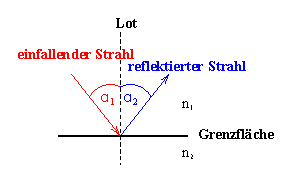
\includegraphics[height=4cm]{Reflexiontheo.pdf}
    \caption{Schematische Darstellung der Reflexion\cite{ap400}.}
    \label{fig:ReflexionTheo}
\end{figure}
\subsection{Theoretische Grundlagen zur Brechung von EM-Wellen.}
\label{sec:Brechung}
Durch verschiedene Ausbreitungsgeschwindigkeiten in verschiedenen Medien, kommt es zur sogenannten Brechung, welche schematisch in \autoref{fig:BrechungTheo} dargestellt ist.
\begin{figure}
    \centering
    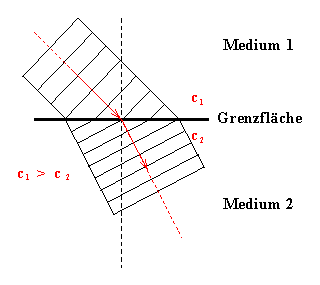
\includegraphics[height = 6cm]{BrechungTheo.pdf}
    \caption{Bildhafte Darstellung einer Brechung einer EM-Welle\cite{ap400}.}
    \label{fig:BrechungTheo}
\end{figure}
Zwischen den beiden Ausbreitungsgeschwindigkeiten $v_1$ und $v_2$ gilt die Beziehung
\begin{equation*}
    \frac{\sin{\alpha}}{\sin{\beta}}= \frac{v_1}{v_2}=\frac{n_2}{n_1}\. .
\end{equation*}
Hier bei ist $\alpha$ der Einfallswinkel, $\beta$ der Brechungswinkel und $n$ der jeweilige Brechungsindex des Materials.
In Luft hat Licht die Ausbreitungsgeschwindigkeit $v_1= 2.9979\cdot 10^8 \frac{\unit{m}}{\unit{s}}$, wobei Luft einen Brechungsindex von 
$n_1= 1.000292$
Diese Richtungsänderung der Elektromagnetischen Welle wird durch das Gesetz von Snellius beschrieben
\begin{equation}
    n_1\sin{\alpha}=n_2sin{\beta}\. .
    \label{eqn:snellius}
\end{equation}

\subsection{Theoretische Grundlagen zur Reflexion und Transmission von EM-Wellen.}
\label{sec: Rfelxion und Transmission}
Natürlicherweise treten an Grenzflächen immer Reflexionen und Transmissionen zeitgleich auf, sodass ein Teil des eintreffenden Lichtes reflektiert $R$ und 
der übrige Teil transmittiert $T$ .
Welchen Anteil des eintreffendes Lichts die jeweilige Aktion hat, ist materialabhängig, jedoch gilt stets $R+T=1$.

\begin{figure}
    \centering
    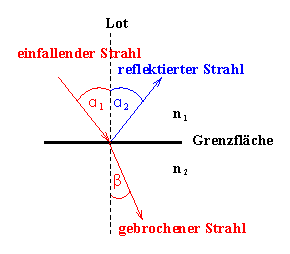
\includegraphics[height= 4cm]{ReflexuTransm.pdf}
    \label{fig:ReflexuTransmTheo}
    \caption{Schematische Darstellung der Reflexion und Transmission\cite{ap400}.}
\end{figure}

\subsection{Theoretische Grundlagen zur Beugung von EM-Wellen.}
\label{sec:BeugungTheo}
Wenn die eine EM-Welle auf ein Objekt trifft, kann häufig beobachtet werden, dass sich diese im Schattenraum ausbreitet.
Also ist die Welle oder in diesem akuten Fall das Licht an Stellen detektierbar, welche es nach der Strahlenoptik nicht erreichen dürft.
Um dieses Phänomen beschreiben zu können, muss die Wellenoptik betrachtet werden.
Eine EM-Welle wird durch ihre Wellenlänge $\lambda$ und ihre Frequenz $\nu$ beschrieben. Wenn es zur Überlagerung mehrerer Wellen kommt, addieren sich die Amplituden
gemäß des Superpositionsprinzip.
Wenn die unterschiedlichen Wellen nun eine Frequenz gemein haben, kann ein Interferenzbild entstehen. Hierbei wird grundsätzlich zwischen destruktiver und konstruktiver Interferenz unterschieden.
Nach dem Huygenschen Prinzip gilt, dass jeder Punkt einer Welle Ausgang einer neuen Elementarwelle ist und die überlagerung dieser eine neue Wellenfront erzeugen.
Trifft eine Welle auf einen Spalt mit Breite $a$, werden alle Punkte in der Spaltöffnung gebeugt und erzeugen so auf einem  Schirm mit Abstand $L$ ein Interferenzmuster.
Die Streifen die konstruktive Interferenz erfahren, erscheinen dann an den Stellen
\begin{equation*}
    a\, \sin{\alpha}=k \lambda  \text{ mit Wellenlänge }\lambda\. .
\end{equation*}
Die Variable $k$ steht hierbei für die Ordnung des Maximums.
Für ein Strichgitter gilt so analog
\begin{equation}
    d\, \sin{\alpha}=k \lambda \. .
    \label{eqn:Gitte}
\end{equation}
Die Größe $d$ wird Gitterkonstante genannt.